\documentclass[10pt]{article}
\usepackage[utf8]{inputenc}
\usepackage[doublespacing]{setspace}
\usepackage{textcomp}
\usepackage{amsmath,amssymb,amsthm}
\usepackage{fancyhdr}
\usepackage{lastpage}
\usepackage[]{hyperref}
\usepackage[pdftex]{graphicx}
\usepackage{ctex}
\usepackage{booktabs}
\usepackage{subfigure}
\usepackage{titlesec}
\usepackage{listings}
\usepackage{enumerate}
\usepackage{bm}
\usepackage{float}
\usepackage{url}
\usepackage[english]{babel}
\usepackage{tikz}
\usepackage{pgfplots}
%\allowdisplaybreaks
\usetikzlibrary{arrows.meta,positioning}
\renewcommand{\contentsname}{\centerline{Contents}}
\pagestyle{fancy}
\author{D}
\def\name{D}
\lhead{ST: Foundations of Deep Learning}
\chead{}
\rhead{\name}
\cfoot{-\space\thepage\space-}
\newtheorem{prob}{\bm{$Problem$}}
\newtheorem{bonus}{\bm{$Bonus\;Problem$}}
\newcommand{\tabincell}[2]{\begin{tabular}{@{}#1@{}}#2\end{tabular}}
\CTEXoptions[today=old]

\begin{document}

\title{Assignment One}
\date{\today}
\maketitle
\thispagestyle{fancy}
\vspace{3mm}

\begin{prob}
\end{prob}
\begin{enumerate}[1)]
\vspace{3mm}

\item
Given the description of the network, firstly we draw its structure.\\
\begin{figure}[H]
\centering
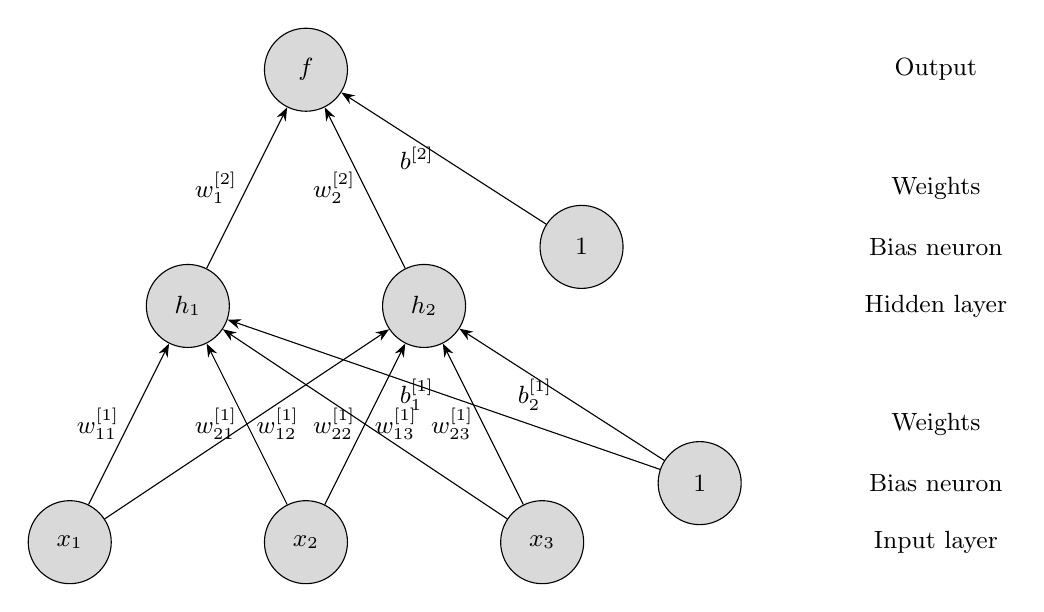
\begin{tikzpicture}[
      mycircle/.style={
         circle,
         draw=black,
         fill=gray,
         fill opacity=0.3,
         text opacity=1,
         inner sep=0pt,
         minimum size=30pt,
         font=\small},
      mytext/.style={
         rectangle,
         font=\small},
      myarrow/.style={-Stealth},
      node distance=1.2cm and 2.4cm
      ]
      \node[mycircle] (c1)at (0,0) {$x_1$};
      \node[mycircle] (c2)at (3,0) {$x_2$};
      \node[mycircle] (c3)at (6,0) {$x_3$};
      \node[mycircle] (c4)at (8,0.75) {$1$};
      \node[mycircle] (c5)at (1.5,3) {$h_1$};
      \node[mycircle] (c6)at (4.5,3) {$h_2$};
      %\node[mycircle] (c7)at (4,2) {$h_2$};
      \node[mycircle] (c8)at (6.5,3.75) {$1$};
      \node[mycircle] (c9)at (3,6) {$f$};
      %\node[mycircle] (c10)at (4,4) {$f_2$};
      \node[mytext] (c21) at (11,0) {Input layer};
      \node[mytext] (c21) at (11,0.75) {Bias neuron};
      \node[mytext] (c21) at (11,1.5) {Weights};
      \node[mytext] (c22) at (11,3) {Hidden layer};
      \node[mytext] (c21) at (11,3.75) {Bias neuron};
      \node[mytext] (c21) at (11,4.5) {Weights};
      \node[mytext] (c21) at (11,6) {Output};
    \foreach \i/\j/\txt/\p in {% start node/end node/text/position
      c1/c5/$w^{[1]}_{11}$/left,
      c1/c6/$w^{[1]}_{21}$/left,
      c2/c5/$w^{[1]}_{12}$/right,
      c2/c6/$w^{[1]}_{22}$/left,
      c3/c5/$w^{[1]}_{13}$/right,
      c3/c6/$w^{[1]}_{23}$/left,
      c4/c5/$b^{[1]}_1$/left,
      c4/c6/$b^{[1]}_2$/left,
      c5/c9/$w^{[2]}_{1}$/left,
      c6/c9/$w^{[2]}_{2}$/left,
      c8/c9/$b^{[2]}$/left}
      %c2.70/c4.290/1/below}
       \draw [myarrow] (\i) -- node[font=\small,\p] {\txt} (\j);
     % draw this outside loop to get proper orientation of 10
     %\draw [myarrow] (c4.250) -- node[sloped,font=\small,above,rotate=180] {10} (c2.110);
\end{tikzpicture}
\caption{Structure of the network}
\end{figure}
Using the given values and functions, we acquire the complete network.\\
\begin{figure}[H]
\centering
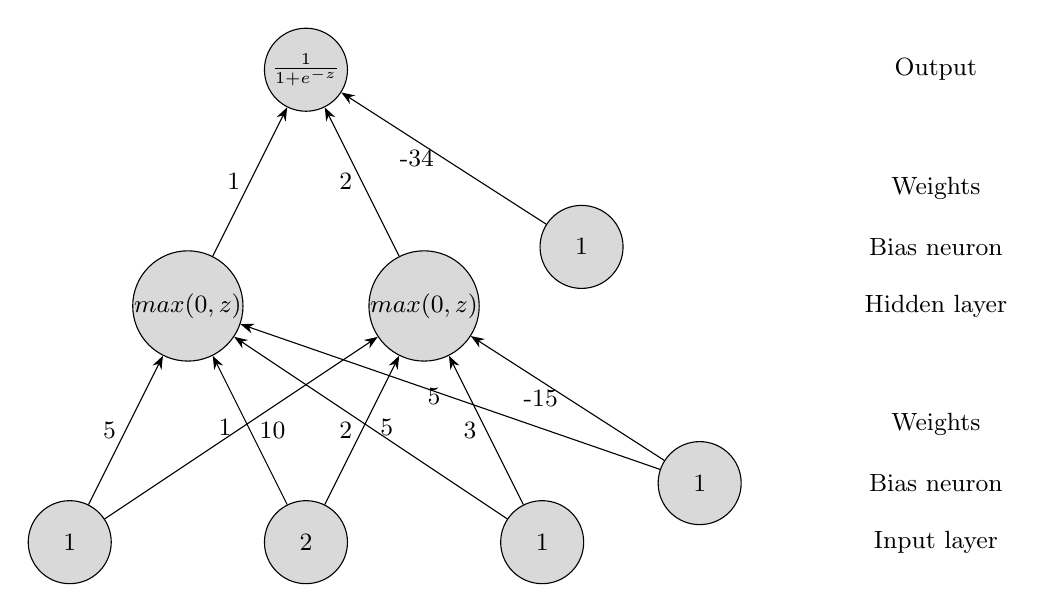
\begin{tikzpicture}[
      mycircle/.style={
         circle,
         draw=black,
         fill=gray,
         fill opacity=0.3,
         text opacity=1,
         inner sep=0pt,
         minimum size=30pt,
         font=\small},
      mytext/.style={
         rectangle,
         font=\small},
      myarrow/.style={-Stealth},
      ]
      \node[mycircle] (c1)at (0,0) {$1$};
      \node[mycircle] (c2)at (3,0) {$2$};
      \node[mycircle] (c3)at (6,0) {$1$};
      \node[mycircle] (c4)at (8,0.75) {$1$};
      \node[mycircle] (c5)at (1.5,3) {$max(0,z)$};
      \node[mycircle] (c6)at (4.5,3) {$max(0,z)$};
      \node[mycircle] (c8)at (6.5,3.75) {$1$};
      \node[mycircle] (c9)at (3,6) {$\frac{1}{1+e^{-z}}$};
      \node[mytext] (c21) at (11,0) {Input layer};
      \node[mytext] (c21) at (11,0.75) {Bias neuron};
      \node[mytext] (c21) at (11,1.5) {Weights};
      \node[mytext] (c22) at (11,3) {Hidden layer};
      \node[mytext] (c21) at (11,3.75) {Bias neuron};
      \node[mytext] (c21) at (11,4.5) {Weights};
      \node[mytext] (c21) at (11,6) {Output};
    \foreach \i/\j/\txt/\p in {
      c1/c5/5/left,
      c1/c6/1/left,
      c2/c5/10/right,
      c2/c6/2/left,
      c3/c5/5/right,
      c3/c6/3/left,
      c4/c5/5/left,
      c4/c6/-15/left,
      c5/c9/1/left,
      c6/c9/2/left,
      c8/c9/-34/left}
       \draw [myarrow] (\i) -- node[font=\small,\p] {\txt} (\j);
\end{tikzpicture}
\caption{Complete network}
\end{figure}
Then the output can be calculated. Firstly we get the sum $\pmb{z}$ in the hidden layer,
\begin{align*}
\pmb{z}&=\pmb{W}^{[1]}\pmb{X}+\pmb{b}^{[1]}\\
&=
  \begin{bmatrix}
    5 & 10 & 5\\
    1 & 2 & 3
  \end{bmatrix}
  \begin{bmatrix}
    1\\
    2\\
    1
  \end{bmatrix}
+
  \begin{bmatrix}
    5\\
    -15
  \end{bmatrix}\\
&=
  \begin{bmatrix}
    30\\
    8
  \end{bmatrix}
+
  \begin{bmatrix}
    5\\
    -15
  \end{bmatrix}\\
&=
  \begin{bmatrix}
    35\\
    -7
  \end{bmatrix}.
\end{align*}
Then input the sum into the activation function and get the outputs $\pmb{h}$ in the hidden layer,
\begin{align*}
\pmb{h}&=g(\pmb{z})\\
&=
  \begin{bmatrix}
    max(0,35)\\
    max(0,-7)
  \end{bmatrix}\\
&=
  \begin{bmatrix}
    35\\
    0
  \end{bmatrix}.
\end{align*}
Repeat the process and get the sum $\pmb{z}'$ in the output layer,
\begin{align*}
\pmb{z}'&=\pmb{W}^{[2]}\pmb{h}+\pmb{b}^{[2]}\\
&=
  \begin{bmatrix}
    1 & 2
  \end{bmatrix}
  \begin{bmatrix}
    35\\
    0
  \end{bmatrix}
+
  \begin{bmatrix}
    -34
  \end{bmatrix}\\
&=
  \begin{bmatrix}
    35
  \end{bmatrix}
+
  \begin{bmatrix}
    -34
  \end{bmatrix}\\
&=
  \begin{bmatrix}
    1
  \end{bmatrix}.
\end{align*}
Finally input the sum into the activation function and get the final output $\pmb{f}$,
\begin{align*}
\pmb{f}&=g(\pmb{z}')\\
&=
  \begin{bmatrix}
    \frac{1}{1+e^{-1}}
  \end{bmatrix}\\
&=
  \begin{bmatrix}
    \frac{e}{1+e}
  \end{bmatrix}.
\end{align*}
Or straightforwardly,
\begin{align*}
f&=\frac{1}{1+e^{-(1\times max(0,5\times1+10\times2+5\times1+5\times1)+2\times max(0,1\times1+2\times2+3\times1+(-15)\times1))+(-34)\times1)}}\\
&=\frac{1}{1+e^{-(1\times max(0,35)+2\times max(0,-7))+(-34)\times1)}}\\
&=\frac{1}{1+e^{-1}}\\
&=\frac{e}{1+e}\\
&\approx0.7311.
\end{align*}
Therefore, $\frac{e}{1+e}$ or 0.7311 is the required result.

\end{enumerate}
\vspace{3mm}

\begin{prob}
\end{prob}
\begin{enumerate}[1)]
\vspace{3mm}

\item
Let $\pmb{w}$ be a vector, where $\pmb{w}=
  \begin{bmatrix}
    w_1 & w_2
  \end{bmatrix}^\top\in\mathbb{R}^2$. Then we get the following graphs.\\
\begin{figure}[H]
\centering
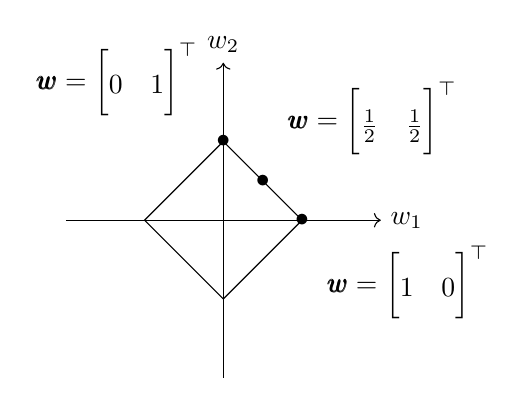
\begin{tikzpicture}
      \draw[->] (-2,0) -- (2,0) node[right] {$w_1$};
      \draw[->] (0,-2) -- (0,2) node[above] {$w_2$};
      \draw (1,0) -- (0,1) -- (-1,0) -- (0,-1) -- (1,0);
      \node[label={315:$\pmb{w}=\begin{bmatrix}
        1 & 0
      \end{bmatrix}^\top$}] at (1,0) {$\bullet$};
      \node[label={135:$\pmb{w}=\begin{bmatrix}
        0 & 1
      \end{bmatrix}^\top$}] at (0,1) {$\bullet$};
      \node[label={45:$\pmb{w}=\begin{bmatrix}
        \frac{1}{2} & \frac{1}{2}
      \end{bmatrix}^\top$}] at (0.5,0.5) {$\bullet$};
\end{tikzpicture}
\caption{Unit norm ball for the 1-norm in $\mathbb{R}^2$, $B_1=\{w\in\mathbb{R}^2,\sum^2_{i=1}|w_i|\leq1\}$}
\end{figure}
\begin{figure}[H]
\centering
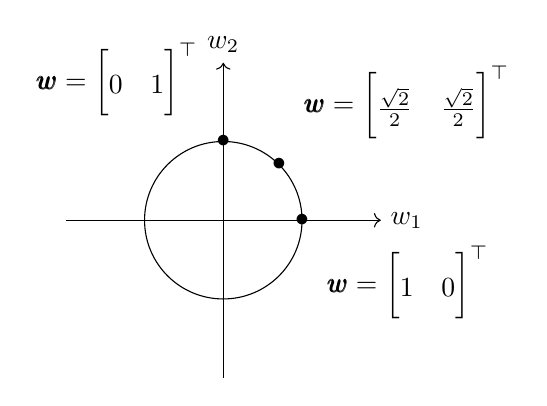
\begin{tikzpicture}
      \draw[->] (-2,0) -- (2,0) node[right] {$w_1$};
      \draw[->] (0,-2) -- (0,2) node[above] {$w_2$};
      \draw (0,0) circle (1);
      \node[label={315:$\pmb{w}=\begin{bmatrix}
        1 & 0
      \end{bmatrix}^\top$}] at (1,0) {$\bullet$};
      \node[label={135:$\pmb{w}=\begin{bmatrix}
        0 & 1
      \end{bmatrix}^\top$}] at (0,1) {$\bullet$};
      \node[label={45:$\pmb{w}=\begin{bmatrix}
        \frac{\sqrt{2}}{2} & \frac{\sqrt{2}}{2}
      \end{bmatrix}^\top$}] at (0.7071,0.7071) {$\bullet$};
\end{tikzpicture}
\caption{Unit norm ball for the 2-norm in $\mathbb{R}^2$, $B_2=\{w\in\mathbb{R}^2,\sum^2_{i=1}(w_i)^2\leq1\}$}
\end{figure}
\begin{figure}[H]
\centering
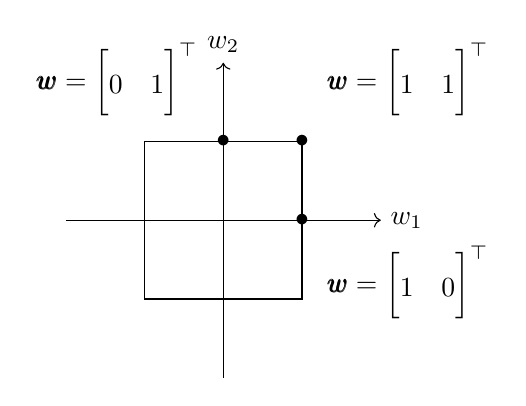
\begin{tikzpicture}
      \draw[->] (-2,0) -- (2,0) node[right] {$w_1$};
      \draw[->] (0,-2) -- (0,2) node[above] {$w_2$};
      \draw (-1,-1) rectangle (1,1);
      %\node[label={135:$(0,1)$}] at (0,1) {$\bullet$};
      %\node[label={0:$(1,1)$}] at (1,1) {$\bullet$};
      \node[label={315:$\pmb{w}=\begin{bmatrix}
        1 & 0
      \end{bmatrix}^\top$}] at (1,0) {$\bullet$};
      \node[label={135:$\pmb{w}=\begin{bmatrix}
        0 & 1
      \end{bmatrix}^\top$}] at (0,1) {$\bullet$};
      \node[label={45:$\pmb{w}=\begin{bmatrix}
        1 & 1
      \end{bmatrix}^\top$}] at (1,1) {$\bullet$};
\end{tikzpicture}
\caption[Caption for LOF]{Unit norm ball for the $\infty$-norm in $\mathbb{R}^2$, $B_\infty=\{w\in\mathbb{R}^2,\forall i\in[1,2], |w_i|\leq1\}$\protect\footnotemark}
\end{figure}
\footnotetext{\;Steinbeck, J. (2016). \textit{Answer to unit ball with p norm in $\mathbb{R}^3$ space}. Retrieved from \url{https://math.stackexchange.com/questions/1631793/unit-ball-with-p-norm-in-mathbbr3-space}.}
Let $\pmb{w}$ be a vector, where $\pmb{w}=
  \begin{bmatrix}
    w_1 & w_2 & w_3
  \end{bmatrix}^\top\in\mathbb{R}^3$. Then we get the following graphs.\\
\begin{figure}[H]
\centering
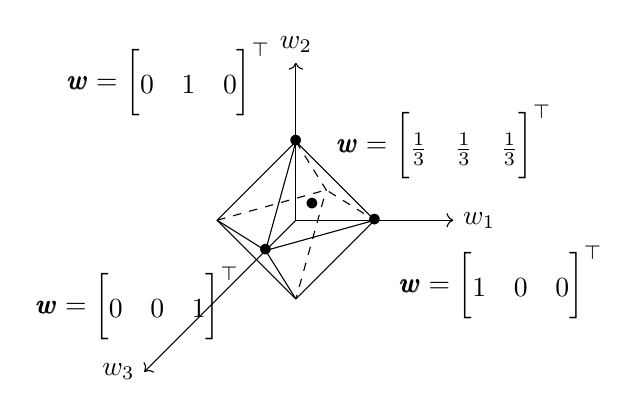
\begin{tikzpicture}
      \draw[->] (0,0,0) -- (2,0,0) node[right] {$w_1$};
      \draw[->] (0,0,0) -- (0,2,0) node[above] {$w_2$};
      \draw[->] (0,0,0) -- (0,0,5) node[left] {$w_3$};
      \draw (0,1,0) -- (1,0,0) -- (0,-1,0);
      \draw (0,1,0) -- (0,0,1) -- (0,-1,0);
      \draw[dashed] (0,1,0) -- (0,0,-1) -- (0,-1,0);
      \draw (0,1,0) -- (-1,0,0) -- (0,-1,0);
      \draw (1,0,0) -- (0,0,1) -- (-1,0,0);
      \draw[dashed] (-1,0,0) -- (0,0,-1) -- (1,0,0);
      \node[label={315:$\pmb{w}=\begin{bmatrix}
        1 & 0 & 0
      \end{bmatrix}^\top$}] at (1,0,0) {$\bullet$};
      \node[label={135:$\pmb{w}=\begin{bmatrix}
        0 & 1 & 0
      \end{bmatrix}^\top$}] at (0,1,0) {$\bullet$};
      \node[label={202.5:$\pmb{w}=\begin{bmatrix}
        0 & 0 & 1
      \end{bmatrix}^\top$}] at (0,0,1) {$\bullet$};
      \node[label={45:$\pmb{w}=\begin{bmatrix}
        \frac{1}{3} & \frac{1}{3} & \frac{1}{3}
      \end{bmatrix}^\top$}] at (0.3333,0.3333,0.3333) {$\bullet$};
\end{tikzpicture}
\caption{Unit norm ball for the 1-norm in $\mathbb{R}^3$, $B_1=\{w\in\mathbb{R}^3,\sum^3_{i=1}|w_i|\leq1\}$}
\end{figure}
\begin{figure}[H]
\centering
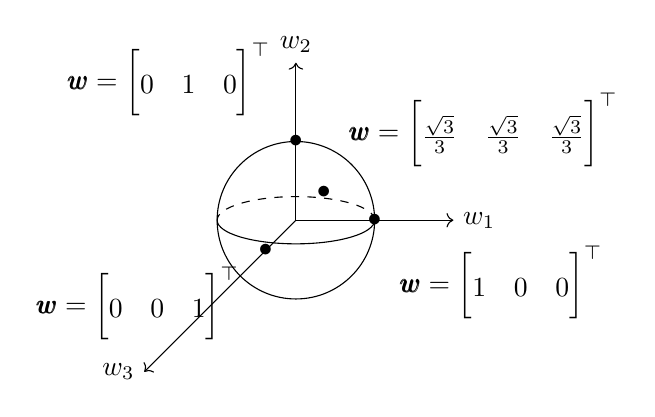
\begin{tikzpicture}
      \draw[->] (0,0,0) -- (2,0,0) node[right] {$w_1$};
      \draw[->] (0,0,0) -- (0,2,0) node[above] {$w_2$};
      \draw[->] (0,0,0) -- (0,0,5) node[left] {$w_3$};
      \draw (0,0) circle (1);
      \draw (-1,0) arc (180:360:1 and 0.3);
      \draw[dashed] (1,0) arc (0:180:1 and 0.3);
      \node[label={315:$\pmb{w}=\begin{bmatrix}
        1 & 0 & 0
      \end{bmatrix}^\top$}] at (1,0,0) {$\bullet$};
      \node[label={135:$\pmb{w}=\begin{bmatrix}
        0 & 1 & 0
      \end{bmatrix}^\top$}] at (0,1,0) {$\bullet$};
      \node[label={202.5:$\pmb{w}=\begin{bmatrix}
        0 & 0 & 1
      \end{bmatrix}^\top$}] at (0,0,1) {$\bullet$};
      \node[label={45:$\pmb{w}=\begin{bmatrix}
        \frac{\sqrt{3}}{3} & \frac{\sqrt{3}}{3} & \frac{\sqrt{3}}{3}
      \end{bmatrix}^\top$}] at (0.57735,0.57735,0.57735) {$\bullet$};
\end{tikzpicture}
\caption{Unit norm ball for the $2$-norm in $\mathbb{R}^3$, $B_2=\{w\in\mathbb{R}^3,\sum^3_{i=1}(w_i)^2\leq1\}$}
\end{figure}
\begin{figure}[H]
\centering
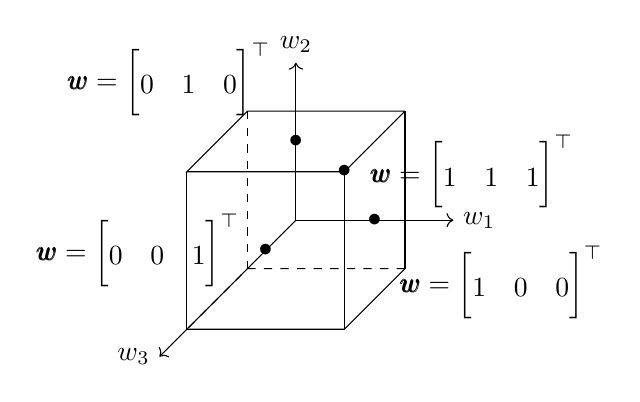
\begin{tikzpicture}
      \draw[->] (0,0,0) -- (2,0,0) node[right] {$w_1$};
      \draw[->] (0,0,0) -- (0,2,0) node[above] {$w_2$};
      \draw[->] (0,0,0) -- (0,0,4.5) node[left] {$w_3$};
      \draw (1,1,-1) -- (-1,1,-1) -- (-1,1,1) -- (1,1,1) -- (1,1,-1);
      \draw (-1,1,1) -- (-1,-1,1);
      \draw (1,1,1) -- (1,-1,1);
      \draw (1,1,-1) -- (1,-1,-1);
      \draw[dashed] (-1,1,-1) -- (-1,-1,-1);
      \draw[dashed] (1,-1,-1) -- (-1,-1,-1) -- (-1,-1,1);
      \draw (-1,-1,1) -- (1,-1,1) -- (1,-1,-1);
      \node[label={315:$\pmb{w}=\begin{bmatrix}
        1 & 0 & 0
      \end{bmatrix}^\top$}] at (1,0,0) {$\bullet$};
      \node[label={135:$\pmb{w}=\begin{bmatrix}
        0 & 1 & 0
      \end{bmatrix}^\top$}] at (0,1,0) {$\bullet$};
      \node[label={180:$\pmb{w}=\begin{bmatrix}
        0 & 0 & 1
      \end{bmatrix}^\top$}] at (0,0,1) {$\bullet$};
      \node[label={0:$\pmb{w}=\begin{bmatrix}
        1 & 1 & 1
      \end{bmatrix}^\top$}] at (1,1,1) {$\bullet$};
\end{tikzpicture}
\caption{Unit norm ball for the $\infty$-norm in $\mathbb{R}^3$, $B_\infty=\{w\in\mathbb{R}^3,\forall i\in[1,3],|w_i|\leq1\}$}
\end{figure}
Unit norm balls in four and more dimensions are omitted.\\

\item
The following diagrams show convex sets.\\
\begin{figure}[H]
\centering
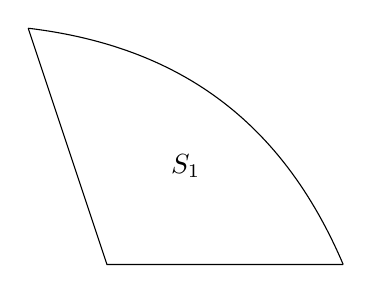
\begin{tikzpicture}
      \draw (-1,3) -- (0,0) -- (3,0);
      \draw (-1,3) to [bend left=30] (3,0);
      \node at (1,1.25) {$S_1$};
\end{tikzpicture}
\caption{Convex set $S_1$}
\end{figure}
\begin{figure}[H]
\centering
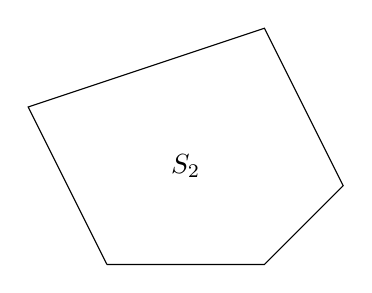
\begin{tikzpicture}
      \draw (0,0) -- (2,0) -- (3,1) -- (2,3) -- (-1,2) -- (0,0);
      \node at (1,1.25) {$S_2$};
\end{tikzpicture}
\caption{Convex set $S_2$}
\end{figure}
\begin{figure}[H]
\centering
\begin{tikzpicture}
      \draw (0,0) to [bend right=40] (6,0);
      \draw (6,0) to [bend right=40] (0,0);
      \node at (3,0) {$S_3$};
\end{tikzpicture}
\caption{Convex set $S_3$}
\end{figure}

\item
The following diagrams show non-convex sets.\\
\begin{figure}[H]
\centering
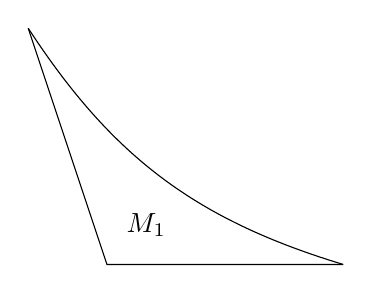
\begin{tikzpicture}
      \draw (-1,3) -- (0,0) -- (3,0);
      \draw (-1,3) to [bend right=20] (3,0);
      \node at (0.5,0.5) {$M_1$};
\end{tikzpicture}
\caption{Non-convex set $M_1$}
\end{figure}
\begin{figure}[H]
\centering
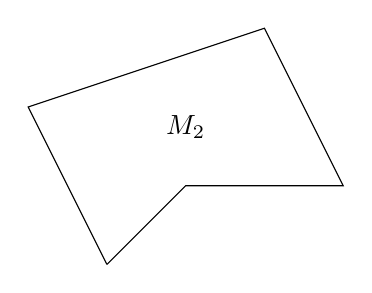
\begin{tikzpicture}
      \draw (0,0) -- (1,1) -- (3,1) -- (2,3) -- (-1,2) -- (0,0);
      \node at (1,1.75) {$M_2$};
\end{tikzpicture}
\caption{Non-convex set $M_2$}
\end{figure}
\begin{figure}[H]
\centering
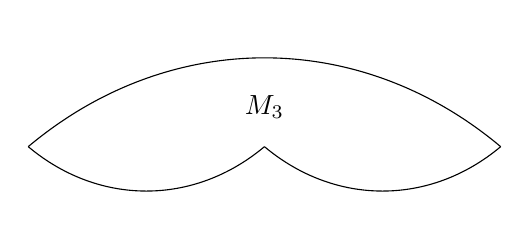
\begin{tikzpicture}
      \draw (0,0) to [bend right=40] (3,0);
      \draw (3,0) to [bend right=40] (6,0);
      \draw (6,0) to [bend right=40] (0,0);
      \node at (3,0.5) {$M_3$};
\end{tikzpicture}
\caption{Non-convex set $M_3$}
\end{figure}

\item
Simply, $f(x)=x^2$ on $\mathbb{R}$ satisfies the condition.\\
\begin{figure}[H]
\centering
\begin{tikzpicture}
   \begin{axis}[
    axis lines = middle,
    xlabel = $x$,
    ylabel = ${f(x)}$,
    colormap/blackwhite
    ]
    \addplot[colormap/blackwhite] {x^2};
  \end{axis}
\end{tikzpicture}
\caption{Convex function $f(x)=x^2$}
\end{figure}
Broadly, $f(x)=x^a$ on $\mathbb{R}_{++}$, for $a\in(-\infty,0]\cup[1,\infty)$, is convex.\\
Further, quadratic functions in three or more dimensions can be convex.\\
\begin{figure}[H]
\centering
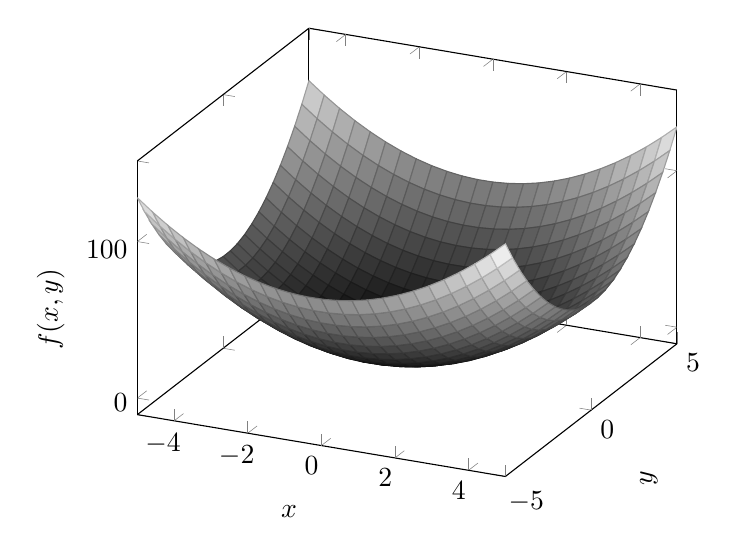
\begin{tikzpicture}
  \begin{axis}[
    axis lines = box,
    xlabel = $x$,
    ylabel = $y$,
    zlabel = {$f(x,y)$},
    colormap/blackwhite
    ]
    \addplot3[surf] {2*x^2+3*y^2+x-y+3};
  \end{axis}
\end{tikzpicture}
\caption{Convex function $f(x,y)=2x^2+3y^2+x-y+3$\protect\footnotemark}
\end{figure}
\footnotetext{\;Eriksen, E. (2010). \textit{Lecture 4 quadratic forms and convexity}. Retrieved from \url{https://www.dr-eriksen.no/teaching/GRA6035/2010/lecture4.pdf}.}

\end{enumerate}
\vspace{3mm}

\begin{prob}
\end{prob}
\begin{enumerate}[1)]
\vspace{3mm}

\item
The gradient is
\begin{align}
\nabla f(w_1,w_2)&=
  \begin{bmatrix}
    \frac{\partial f}{\partial w_1}\\
    \frac{\partial f}{\partial w_2}
  \end{bmatrix}\\
&=
  \begin{bmatrix}
    2.5w_1+15\\
    2w_2-16
  \end{bmatrix}.
\end{align}
\vspace{3mm}

\item
The Hessian is
\begin{align}
\nabla^2f(w_1,w_2)&=
  \begin{bmatrix}
    \frac{\partial^2 f}{\partial w_1^2} & \frac{\partial ^2 f}{\partial w_1\partial w_2}\\
    \frac{\partial^2 f}{\partial w_2\partial w_1} & \frac{\partial^2 f}{\partial w_2^2}
  \end{bmatrix}\\
&=
  \begin{bmatrix}
    2.5 & 0\\
    0 & 2
  \end{bmatrix}.
\end{align}
\vspace{3mm}

\item
The necessary conditions for a minimizers $\pmb{w}^*=
  \begin{bmatrix}
    w_1^* & w_2^*
  \end{bmatrix}^\top$ are
\begin{align}
&\nabla f(\pmb{w}^*)=0,\\
&\nabla^2f(\pmb{w}^*)\geq0.
\end{align}
Further in (5),
\begin{align}
\nabla f(w_1,w_2)&=
  \begin{bmatrix}
    \frac{\partial f}{\partial w_1}\\
    \frac{\partial f}{\partial w_2}
  \end{bmatrix}\\
&=
  \begin{bmatrix}
    2.5w_1+15\\
    2w_2-16
  \end{bmatrix}\\
&=
  \begin{bmatrix}
    0\\
    0
  \end{bmatrix},
\end{align}
thus $w_1=-6$ and $w_2=8$.\\
Further in (6), let $\lambda$ be the eigenvalues of the Hessian,
\begin{align}
det(
  \begin{bmatrix}
    2.5 & 0\\
    0 & 2
  \end{bmatrix}
-\lambda
  \begin{bmatrix}
    1 & 0\\
    0 & 1
  \end{bmatrix}
)=0,
\end{align}
thus $\lambda_1=2.5$ and $\lambda_2=2$, so $\lambda_1\geq0$ and $\lambda_2\geq0$.\\

\item
Given the previous result, we have the optimal solution $
  \begin{bmatrix}
    -6 & 8
  \end{bmatrix}^\top$\\
and $\smash{\displaystyle\min_{\pmb{w}}}f(w_1,w_2)=0$.\\

\item
Straightforwardly,
\begin{align}
f(x_1,x_2)&=1.25(w_1+6)^2+(w_2-8)^2\\
&=[\frac{\sqrt{5}}{2}(w_1+6)]^2+(w_2-8)^2\\
&=(\frac{\sqrt{5}}{2}w_1+3\sqrt{5})^2+(w2-8)^2\\
&=[\frac{\sqrt{2}}{2}(\frac{2}{\sqrt{2}}\frac{\sqrt{5}}{2}w_1+\frac{2}{\sqrt{2}}3\sqrt{5})]^2+\frac{1}{2}[\frac{2}{\sqrt{2}}(w_2-8)]^2\\
&=\frac{1}{2}(\frac{\sqrt{10}}{2}w_1+3\sqrt{10})^2+\frac{1}{2}(\sqrt{2}w_2-8\sqrt{2})^2.
\end{align}
Let $\pmb{X}=
  \begin{bmatrix}
    \frac{\sqrt{10}}{2} & \sqrt{2}
  \end{bmatrix}^\top$
and $\pmb{y}=
  \begin{bmatrix}
    -3\sqrt{10} & 8\sqrt{2}
  \end{bmatrix}^\top$
, then (15) is expressed as
\begin{align}
f(w_1,w_2)&=\frac{1}{2}||\pmb{X}^\top\pmb{w}-\pmb{y}||^2_2.
\end{align}
Refer to the lecture notes\footnote{\;Tappenden, R. (2020). \textit{Lecture notes in special topic: foundations of deep learning}. Unpublished manuscript.},
\begin{align}
\nabla f(\pmb{w})&=\pmb{X}\pmb{X}^\top\pmb{w}-\pmb{X}\pmb{y},
\end{align}
and given the gradient of $f$ is L-Lipschitz continuous, let $\pmb{w}_a,\pmb{w}_b\in\mathbb{R}^2$ and we have
\begin{align}
||\nabla f(\pmb{w}_a)-\nabla f(\pmb{w}_b)||_2&\leq L||\pmb{w}_a-\pmb{w}_b||_2\\
\frac{||\nabla f(\pmb{w}_a)-\nabla f(\pmb{w}_b)||_2}{||\pmb{w}_a-\pmb{w}_b||_2}&\leq L.
\end{align}
Combine (17) and (19),
\begin{align}
\frac{||(\pmb{X}\pmb{X}^\top\pmb{w}_a-\pmb{X}\pmb{y})-(\pmb{X}\pmb{X}^\top\pmb{w}_b-\pmb{X}\pmb{y})||_2}{||\pmb{w}_a-\pmb{w}_b||_2}&\leq L.
\end{align}
For the left side of (20),
\begin{align}
\frac{||(\pmb{X}\pmb{X}^\top\pmb{w}_a-\pmb{X}\pmb{y})-(\pmb{X}\pmb{X}^\top\pmb{w}_b-\pmb{X}\pmb{y})||_2}{||\pmb{w}_a-\pmb{w}_b||_2}&=
\frac{||\pmb{X}\pmb{X}^\top(\pmb{w}_a-\pmb{w}_b)||_2}{||\pmb{w}_a-\pmb{w}_b||_2}.
\end{align}
Use the property of matrix norms, $||\pmb{A}\pmb{B}||\leq||\pmb{A}||||\pmb{B}||$,
\begin{align}
\frac{||\pmb{X}\pmb{X}^\top(\pmb{w}_a-\pmb{w}_b)||_2}{||\pmb{w}_a-\pmb{w}_b||_2}\leq
\frac{||\pmb{X}\pmb{X}^\top||_2||\pmb{w}_a-\pmb{w}_b||_2}{||\pmb{w}_a-\pmb{w}_b||_2}.
\end{align}
For the right side of (22),
\begin{align}
\frac{||\pmb{X}\pmb{X}^\top||_2||\pmb{w}_a-\pmb{w}_b||_2}{||\pmb{w}_a-\pmb{w}_b||_2}&=||\pmb{X}\pmb{X}^\top||_2\\
&=||
  \begin{bmatrix}
    \frac{\sqrt{10}}{2}\\
    \sqrt{2}
  \end{bmatrix}
  \begin{bmatrix}
    \frac{\sqrt{10}}{2} & \sqrt{2}
  \end{bmatrix}||_2\\
&=||
  \begin{bmatrix}
    \frac{5}{2} & \sqrt{5}\\
    \sqrt{5} & 2
  \end{bmatrix}||_2\\
&=\sigma_{max}(
  \begin{bmatrix}
    \frac{5}{2} & \sqrt{5}\\
    \sqrt{5} & 2
  \end{bmatrix})\\
&=max(\sqrt{\frac{81}{4}},0)\\
&=\frac{9}{2}.
\end{align}
Combine (22) and (28),
\begin{align}
\frac{||\pmb{X}\pmb{X}^\top(\pmb{w}_a-\pmb{w}_b)||_2}{||\pmb{w}_a-\pmb{w}_b||_2}\leq\frac{9}{2}.
\end{align}
With (20) and (29), we get the range of $L$,
$[\frac{9}{2},\infty)$, and the best Lipschitz constant, $\frac{9}{2}$.

\end{enumerate}
\vspace{3mm}

\begin{prob}
\end{prob}
\begin{enumerate}[1)]
\vspace{3mm}

\item
Plot with Python.\\
\begin{figure}[H]
  \centering
  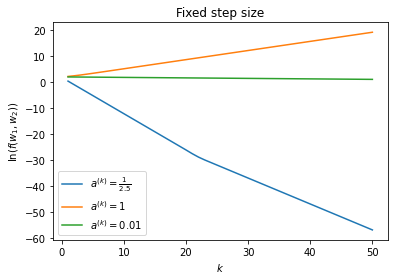
\includegraphics[scale=0.65]{p41a.png}
  \caption{$f(w_1,w_2)$ vs. $k$}
\end{figure}

\item
Plot with Python.\\
\begin{figure}[H]
  \centering
  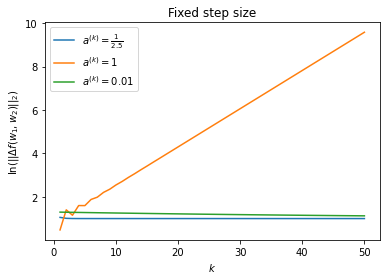
\includegraphics[scale=0.65]{p42a.png}
  \caption{$||\Delta f(w_1,w_2)||_2$ vs. $k$}
\end{figure}

\item
When $a^{(k)}=\frac{1}{2.5}$, the step length is just right; $f(w_1,w_2)$ approaches 0, the global minimum of the function, after 3 iterations and converges; $||\Delta f(w_1,w_2)||_2$ approaches 1, converges and merely changes after 5 iterations.\\
When $a^{(k)}=1$, the step length is too big; $f(w_1,w_2)$ increases and diverges; $||\Delta f(w_1,w_2)||_2$ vibrates from the beginning, increases after 5 iterations and diverges.\\
When $a^{(k)}=0.01$, the step length is too small; $f(w_1,w_2)$ goes to 0 but is still approximately 12 away from 0 after 50 iterations; $||\Delta f(w_1,w_2)||_2$ goes to 1 and has not reached stationary after 50 iterations.\\

\item
Plot with Python.\\
\begin{figure}[H]
  \centering
  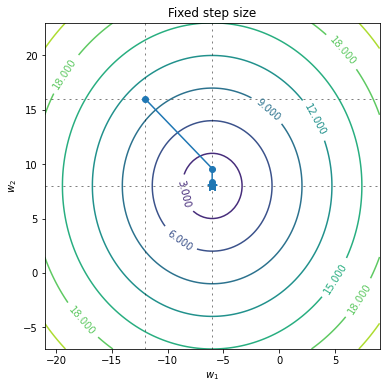
\includegraphics[scale=0.6]{p43a.png}
  \caption{Gradient descent with $a^{(k)}=\frac{1}{2.5}$}
\end{figure}
\begin{figure}[H]
  \centering
  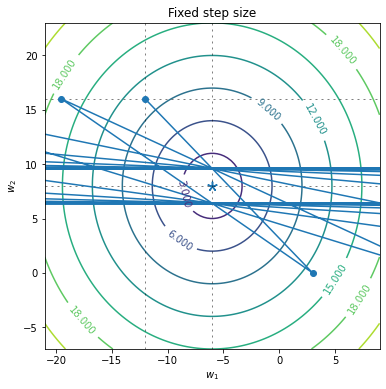
\includegraphics[scale=0.6]{p43b.png}
  \caption{Gradient descent with $a^{(k)}=1$}
\end{figure}
\begin{figure}[H]
  \centering
  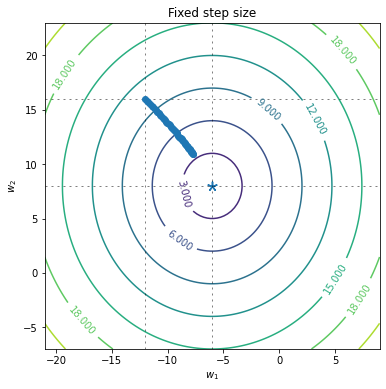
\includegraphics[scale=0.6]{p43c.png}
  \caption{Gradient descent with $a^{(k)}=0.01$}
\end{figure}

\end{enumerate}

\end{document}
